\documentclass[11pt]{article}

\usepackage{a4wide}
\usepackage{mathptm}
\usepackage{xspace}
\usepackage{amsmath}
\usepackage{graphicx}
\usepackage{algorithm}
\usepackage{algpseudocode}
\usepackage{tikz}
\usepackage{tkz-graph}
\usetikzlibrary{shapes.misc, positioning}
\usepackage{listings}
\usepackage{color}

\definecolor{dkgreen}{rgb}{0,0.6,0}
\definecolor{gray}{rgb}{0.5,0.5,0.5}
\definecolor{mauve}{rgb}{0.58,0,0.82}

\lstset{frame=tb,
  language=Java,
  aboveskip=3mm,
  belowskip=3mm,
  showstringspaces=false,
  columns=flexible,
  basicstyle={\small\ttfamily},
  numbers=left,
  numberstyle=\tiny\color{gray},
  keywordstyle=\color{blue},
  commentstyle=\color{dkgreen},
  stringstyle=\color{mauve},
  breaklines=true,
  breakatwhitespace=true,
  tabsize=3
}
\begin{document}

\title{My Best Software Technology Evaluation Project Ever}

\author{Jonatan Valen}

\maketitle

\begin{abstract}

  10-15 lines with the software technology and the highlights from the
  project that has been undertaken.

\end{abstract}

%\input{commands}

\setlength{\parskip}{1em} % Adds vertical space between paragraphs
\setlength{\parindent}{0pt} % Removes the indent at the start of each paragraph

\section{Introduction}
\label{sec:introduction}

\subsection{Development of the Feedback App}
In this project we have developed a feedback app for voting on polls. We have implemented register and login functionality. A user can create polls that are either private or public, and both users and voters can vote on polls. 
Only logged in users can vote on polls. We have also created a pollinfo display where users can look at results of their own polls. On this pollinfo page, you can also find an shareable link so that people that dont have user accounts can vote on public polls. 
Users can also manage their polls by ending them, starting them again, and deleting them. 

\subsection{Technology stack}
The technology stack chosen for this project is both robust and dynamic, encompassing a spectrum of modern development tools and frameworks. 
We have employed React for our front-end development, capitalizing on its component-based architecture for a responsive and interactive user interface. 
The back-end is powered by Spring Boot, providing a strong and scalable foundation for our application services. For message handling and asynchronous operations, RabbitMQ has been integrated, ensuring efficient communication and process management.

Further enhancing our application's capabilities, we have incorporated Tailwind CSS for streamlined styling, JPA (Java Persistence API) for efficient data handling, and Hibernate for object-relational mapping, ensuring a seamless data management experience. 
Firebase is used for our authentication solutions, fortifying the app's security. 
Additionally, Dweet.io has been utilized for its simplicity in real-time messaging, and an H2 database for its lightweight and easy-to-use nature.

\subsection{Results}
During this project, we have gained a better insight into different software technologies, frameworks and tools. 
We now have a working prototype of a voting app which can easily be extendable to include more features in the future. 
\subsection{Overview}
This rest of this report is organised as follows:
Section~\ref{sec:technology} gives an overview of the software technology stack used. 
Section~\ref{sec:design} describes the design of the prototype. 
Section~\ref{sec:implementation} details how the prototype has been implemented. 
Section~\ref{sec:evaluation} explains how the prototype has been tested and what experiments have been done.  
In Section~\ref{sec:conclusion} we provide conclusions regarding different aspects of the project.



\section{Software Technology Stack}
\label{sec:technology}

\subsection{React and Tailwind: Efficient Frontend Development}

We have chosen React and Tailwind for our web application's frontend, aligning with Goadrich and Rogers' findings that React Native excels across different operating systems \cite[p.~611]{goadrich2011smart}. React enables us to build dynamic web applications where data changes without page reloads. Tailwind CSS, a utility-first framework, has been rising in popularity for its streamlined approach to styling.

React stands out for its component-based architecture, allowing developers to create self-contained components managing their own state, leading to reusable, complex UIs. It simplifies development and reduces redundancy. React's lifecycle management offers fine control over component behavior, and its declarative nature means developers describe the UI while React handles DOM updates efficiently. This is especially beneficial for large application maintainability.

The React community is vast, offering numerous libraries and tools like Redux, MobX, and React Router. Developer tools like React Developer Tools enhance the debugging experience, and React's helpful error messages aid in swift issue resolution.

Tailwind CSS complements this by enabling in-HTML styling, reducing the need to switch between HTML and CSS files. Its utility-first approach and self-explanatory classes enhance readability and speed up development. Tailwind's focus on utility classes often results in smaller CSS files, boosting performance. Its JIT compiler ensures minimal CSS generation, enhancing load times and overall web application performance.

\subsection{Spring Boot: Back-End Infrastructure}
Spring Boot is an extension of the Spring framework that simplifies the initial setup and development of new Spring applications.\cite{springboot2023} 
It favors convention over configuration and is designed to get you up and running as quickly as possible. Here's a detailed explanation of why Spring Boot is an excellent choice for our back-end infrastructure:

Spring Boot simplifies the management of application configurations. 
It eliminates the need for defining boilerplate configuration with its auto-configuration feature.
This feature automatically configures your application based on the libraries present on the classpath. 
This can significantly reduce development time and increase productivity because developers can focus on the unique aspects of their application rather than on infrastructure setup. 

Spring Boot makes it easy to create standalone, production-grade Spring-based applications that can be run directly from the command line without requiring an external web server. 
This is made possible by embedding servers like Tomcat, Jetty, or Undertow directly in the application. 
The ability to run as a standalone app simplifies both the development and the deployment processes.

To streamline the configuration process, Spring Boot provides a set of 'starter' dependencies that bundle the necessary libraries to get a feature working. 
These starters cover many Spring Boot features, such as data access, messaging, and web services. 
Using starters, you can avoid library version conflicts and ensure that you're using a set of dependencies that Spring Boot has tested and approved.

Spring Boot benefits from the strong support of the vibrant and extensive Spring community. 
There are numerous guides, tutorials, and a comprehensive reference documentation available. 
Moreover, the community support forums and Stack Overflow are active and helpful in solving problems.

Spring Boot has excellent integration with Spring Data, which simplifies database access and provides support for various data access technologies, including JPA, JDBC, and NoSQL. 
Spring Boot also works well with Hibernate - one of the most popular ORM tools - making it easier to work with databases using an object-oriented paradigm.

\subsection{RabbitMQ and Dweet.io: Message Systems}

RabbitMQ, an open-source message broker, is chosen for its reliability, scalability, and flexibility in handling application messaging systems.\cite{RabbitamqpSpec} It serves as a platform-neutral intermediary, enabling asynchronous communication between services with support for various messaging protocols, intricate queuing, and multiple exchange types. This ensures flexible routing and enhances system robustness by allowing producers and consumers to scale independently. Additionally, RabbitMQ's features like message durability, persistent queues, and capability to operate in high-load environments with consistent hashing and sharding make it ideal for maintaining application integrity and managing high message volumes.

Complementing RabbitMQ, Dweet.io offers a simplified solution for real-time messaging, especially beneficial for Internet of Things (IoT) applications. It enables devices to "dweet" messages for instant access by subscribed clients, emphasizing timely data delivery with minimal setup requirements. This makes Dweet.io highly accessible for immediate deployment and integration.

Together, RabbitMQ and Dweet.io provide a comprehensive messaging solution. RabbitMQ handles the heavy-duty, reliable queuing and processing of messages, while Dweet.io contributes with its real-time messaging capabilities, ensuring a responsive and interconnected application ecosystem.



\subsection{JPA, Hibernate and H2: Data Management and Storing}

Java Persistence API (JPA) is a Java specification providing an Object-Relational Mapping (ORM) standard. 
This abstraction simplifies the interaction between Java objects and relational databases. 
JPA's primary advantage lies in its database-agnostic nature, offering flexibility in database choice and minimal application code changes when switching databases.

Hibernate, as an implementation of JPA, enhances its capabilities. 
It's renowned for its performance optimization features, such as lazy loading and sophisticated caching mechanisms. 
Hibernate also supports a rich set of querying capabilities through the Hibernate Query Language (HQL) and Criteria API, enabling more complex and efficient data retrieval operations. 
According to a study presented at the 2021 23rd International Conference on Control Systems and Computer Science, "ORM (object/relational mapping) has now widespread. This is mainly due to Hibernate, an open-source ORM, and Spring Data, an umbrella project from the Spring family whose purpose is to unify and facilitate access to different kinds of persistence stores, including relational database systems and NoSQL databases" \cite{orm2021cscs}.
Together, JPA and Hibernate offer:

\begin{itemize}
  \item \textbf{Simplified Database Interactions}: By abstracting complex JDBC operations, they reduce boilerplate code and streamline database interactions.
  \item \textbf{Advanced Query Capabilities}: Enhanced querying and retrieval options facilitate sophisticated data handling.
  \item \textbf{Performance Optimizations}: Features like caching and batching improve application performance and database interaction efficiency.
\end{itemize}

The H2 database is an in-memory, Java-based database known for its speed and simplicity. 
Primarily used in development and testing environments, H2 stands out for its ease of setup and rapid execution. 
It offers a web console for direct database interactions, enhancing its usability during development.




\subsection{Firebase: Authentication (New Technology)}

Firebase Authentication provides a full backend service that can authenticate users through multiple methods, including passwords, phone numbers, popular federated identity providers like Google, Facebook, and Twitter, and more. The decision to use Firebase for authentication in the application is based on its comprehensive suite of features that enhance user security and improve the overall user experience.

Firebase Authentication offers a seamless integration with applications, providing a complete identity solution supporting email/password auth, social media login, and phone authentication. Its SDKs and ready-made UI libraries allow for quick implementation of secure user authentication.

The service not only handles user authentication but also manages user accounts and sessions with ease. It's equipped with features such as email and password reset, account verification, and sign-in link capabilities, which contribute to a robust authentication flow.

According to Pramono and Javista, Firebase Authentication ensures that user credentials are securely managed and stored, preventing users from manipulating data or using the identity of another user due to its security and strict data verification process \cite{pramono2021firebase}. The platform is compliant with identity standards such as OAuth 2.0 and OpenID Connect, so user data is handled in a secure and standardized manner.

Designed to handle large-scale applications, Firebase Authentication can effortlessly scale to accommodate millions of users. The flexibility offered by Firebase allows developers to focus on the user experience while Firebase takes care of the authentication backend.

Firebase Authentication is part of the larger Firebase ecosystem, which means it can be easily integrated with other Firebase services like Firestore, Firebase Realtime Database, and Firebase Cloud Functions. This integration provides a seamless development experience and allows for the creation of sophisticated, authenticated workflows.

By incorporating Firebase Authentication, the application streamlines the user sign-in process and ensures that authentication is handled safely and efficiently, allowing developers to focus on building features that add value to the user experience rather than the intricacies of user security management.


\section{Design}
\label{sec:design}

The application is designed using modern scalable technologies with clear separation of concerns across its various layers. 
The system is built upon a microservices architecture pattern, enabling independent scaling and flexibility in deployment


\begin{figure}[!htbp]
\centering
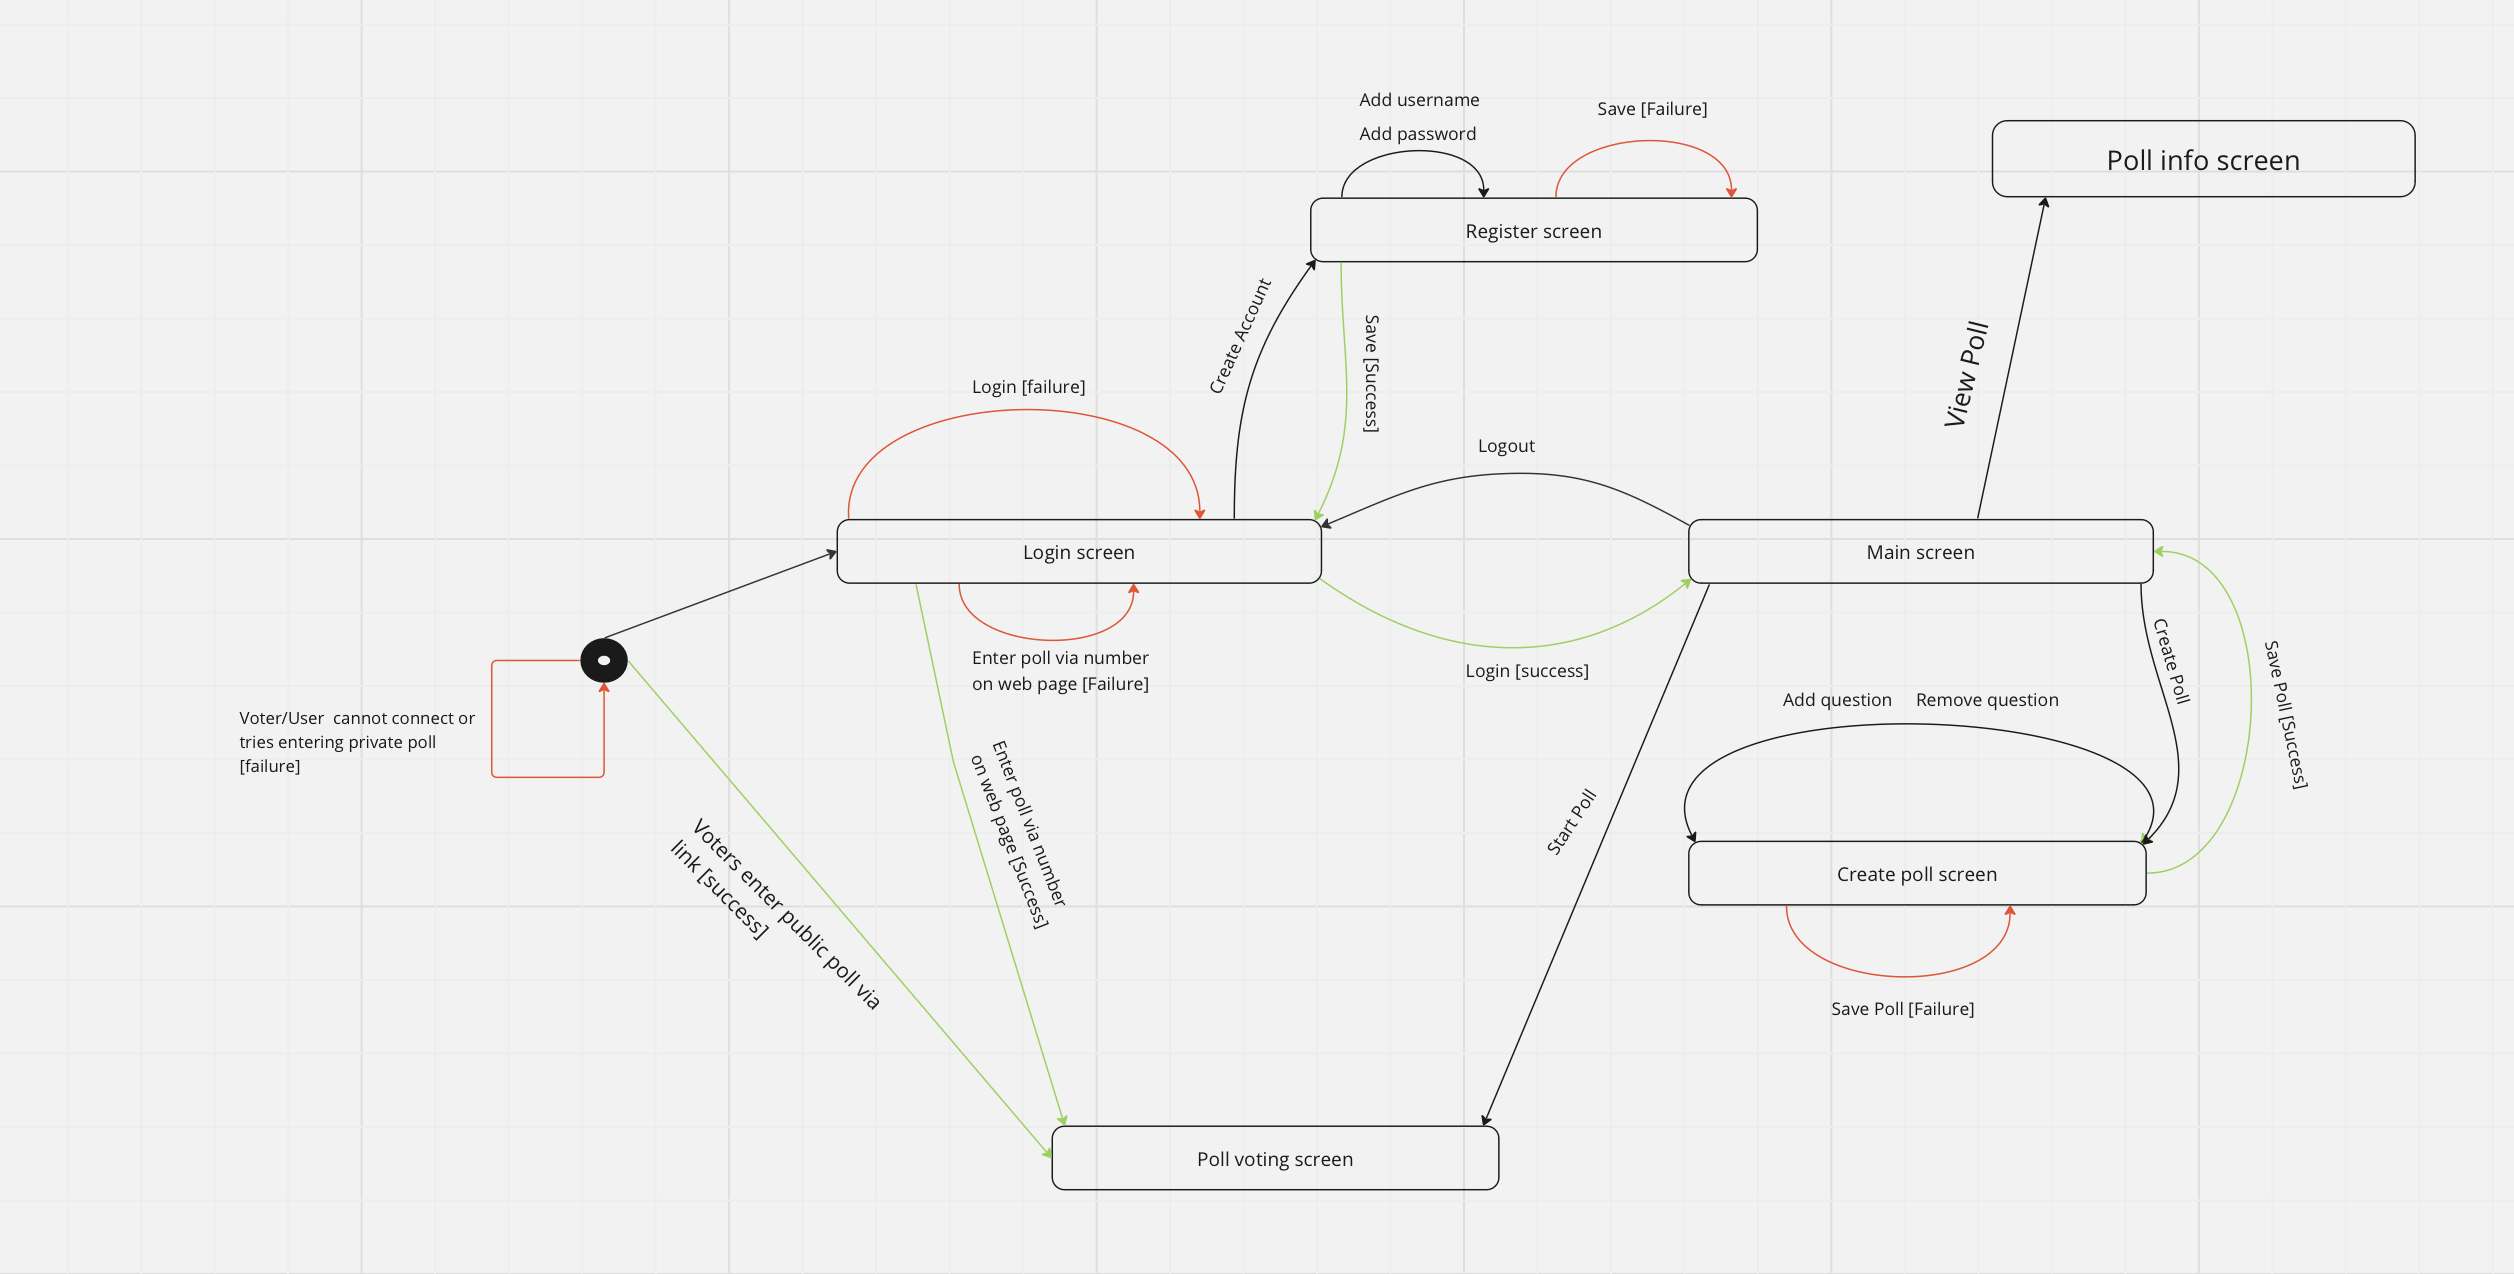
\includegraphics[width=\linewidth]{figs/ApplicationFlowDiagram.png}
\caption{Application flow diagram}
\label{fig:appflow}
\end{figure}

The application flow diagram, as seen in Figure~\ref{fig:appflow}, provides a high-level overview of the users journey through the application. It begins with the Login screen, where users can either log in or register. In case of registration, the user is prompted to add a username and password before being redirected to the main screen upon successful account creation. The main screen serves as a navigation hub, allowing users to view polls, create new polls, or log out.

Upon selecting a poll, the user is taken to the Poll Voting screen, where they can cast their vote. Both successful and unsuccessful actions within the application are accounted for, with clear pathways leading the user to appropriate screens or error messages, ensuring a robust user experience. The diagram distinctly marks the paths taken during normal operation (success) and exceptions (failure), reflecting the applications error-handling capabilities.

The flow for creating a poll is similarly user-friendly, with the Create Poll screen allowing users to add or remove questions before saving. The user is provided with immediate feedback on the success or failure of their actions, with the system guiding them accordingly.

In addition to the primary user flows, the diagram also highlights potential failure states, such as login failures or issues entering private polls, indicating comprehensive error handling throughout the application.
    


\begin{figure}[!htbp]
\centering
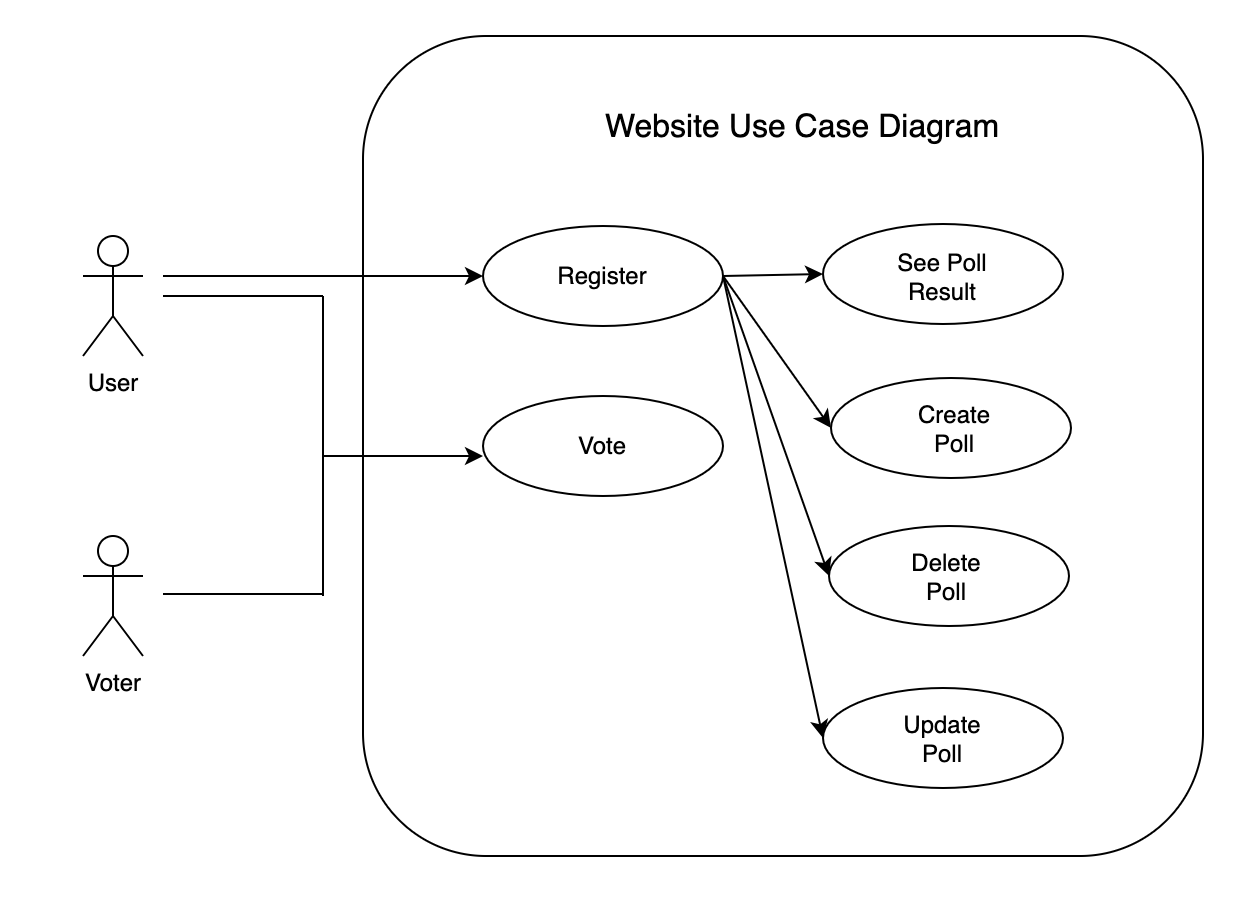
\includegraphics[width=0.5\linewidth]{figs/UserDiagram.png}
\caption{Website use case diagram}
\label{fig:userdiagram}
\end{figure}

Figure~\ref{fig:userdiagram} delineates the use case diagram for the website, detailing the interactions that both 'User' and 'Voter' actors have with the system. The 'User' actor, representing registered individuals, has the capabilities to register, vote, see poll results, create, delete, and update polls. The distinction between a general 'User' and a 'Voter' highlights the specialized role that a 'Voter' plays in the context of the application, primarily focused on the voting functionality. The use case diagram clearly identifies the system's boundary and the primary functions available to the users, providing a straightforward visualization of the different ways the users can interact with the system. It serves as a guide for understanding the user requirements and the scope of the system from an end-user perspective


\begin{figure}[!htbp]
\centering
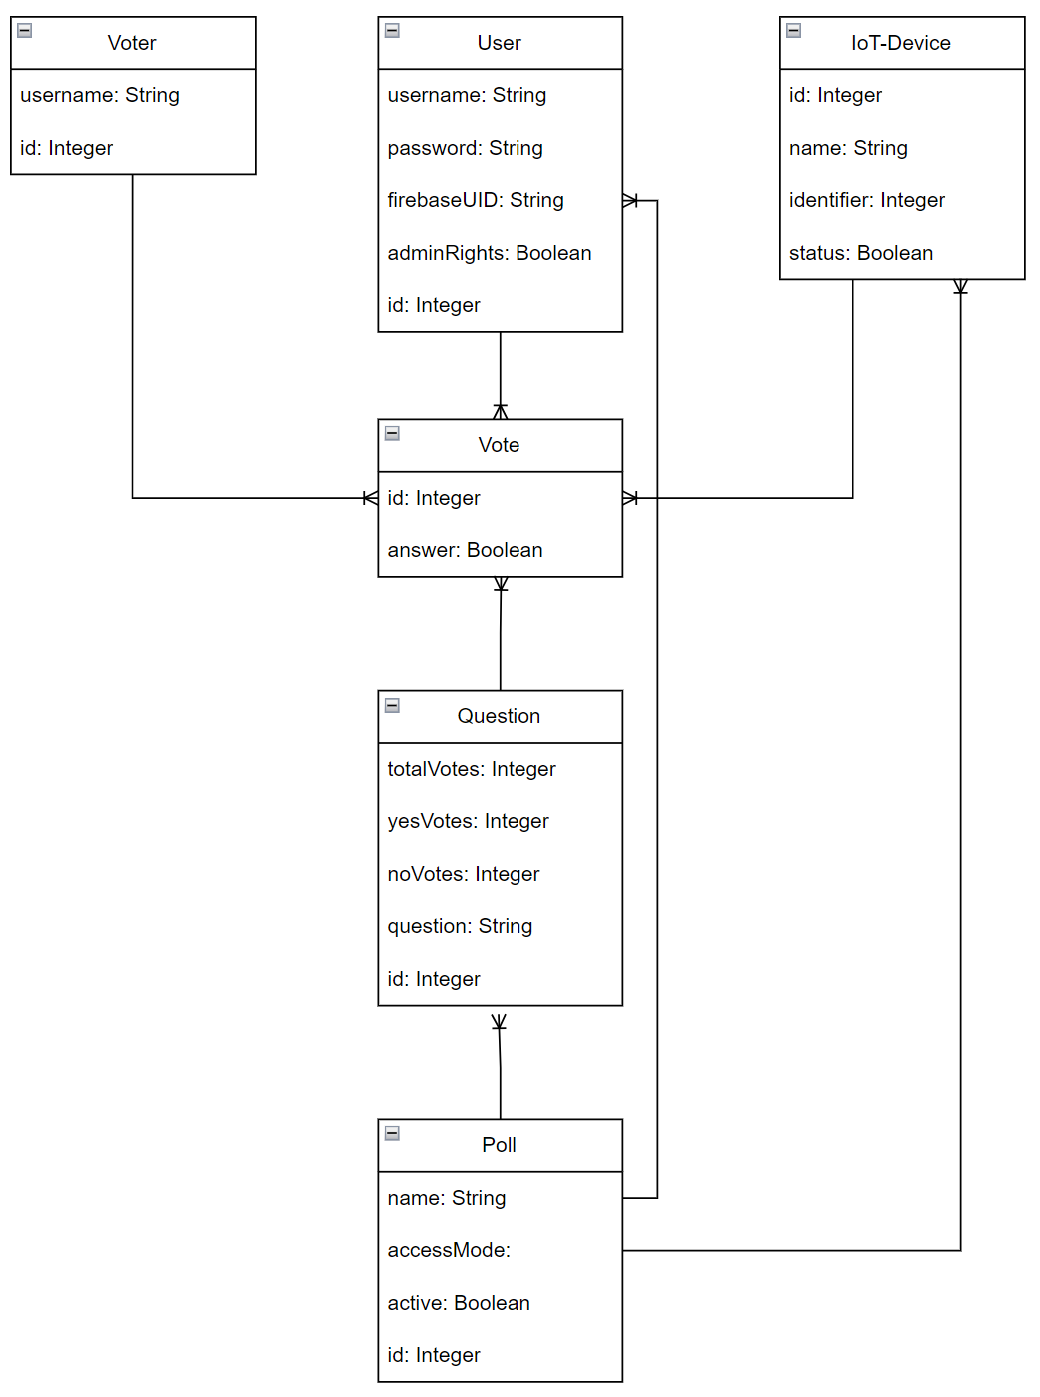
\includegraphics[width=0.4\linewidth]{figs/DomainModel.png}
\caption{Domain model}
\label{fig:domainmodel}
\end{figure}

Figure~\ref{fig:domainmodel} presents the domain model of the application, illustrating the primary entities and their relationships. The model defines a User entity with attributes for username, password, a unique Firebase user ID, administrative rights, and an identifier. This entity is central to the model and is associated with Voter, Vote, and IoT-Device entities.

The Voter is a specialized type of User, indicated by a shared id attribute, encapsulating only the necessary attributes for voting purposes, such as username and voter identifier. The Vote entity represents an individual vote, with a boolean answer attribute and a unique identifier, which is associated with a Question. Each Question contains attributes for the total number of votes, counts of yes and no votes, the text of the question, and an identifier.

The model also includes a Poll entity, which aggregates Questions. It has attributes for the poll name, access mode, an active status indicator, and an identifier. The IoT-Device entity represents devices that may interact with the system, characterized by an identifier, a name, another unique identifier, and a status boolean, which could be used for integrating IoT capabilities within the application.

This domain model serves as a blueprint for the systems structure, outlining the key data elements and their interconnections, which are crucial for understanding the relationships and data flow within the application.

\subsection{Design Patterns}

\subsubsection{Model-View-Controller (MVC)}

Our application employs the \textbf{Model-View-Controller (MVC)} design pattern, a paradigm for creating software with separated concerns, enhancing code reusability, and facilitating parallel development. The implementation of MVC within our voting application is outlined as follows:

\begin{description}
  \item[Model:] The model layer manages data and business logic. It encompasses domain entities corresponding to database tables, abstracting database access through Spring Data JPA with Hibernate. The models, defined as POJOs, encapsulate the application's data structures and business rules.
  
  \item[View:] Implemented using React.js, the View is a dynamic user interface for client-side interactions. Tailwind CSS is integrated for responsive and aesthetic styling. The frontend operates independently, interfacing with the server through API calls.
  
  \item[Controller:] Controllers in the `controller` package mediate between Model and View, handling HTTP requests with `@RestController` annotations. They direct user inputs to model operations and return appropriate responses, whether as rendered views or data payloads.
\end{description}

\paragraph{Advantages of MVC in Our Application:}
\begin{itemize}
  \item \textbf{Separation of Concerns:} MVC facilitates maintenance and scalability with its independent component operation.
  \item \textbf{Parallel Development:} Developers can work on the Model, View, and Controller concurrently, expediting development cycles.
  \item \textbf{Testability:} The separation allows for precise automated testing of business logic and user interfaces.
  \item \textbf{Adaptability:} Business logic or UI changes incur minimal impact on the overall architecture.
\end{itemize}

The MVC design pattern is integral to our application's design, ensuring a clean separation between user interface, business processing, and data management components, making the system robust, maintainable, and adaptable.


\subsection{Architectural Layers}
\subsubsection{Layer (Frontend)}

\begin{itemize}

\item React.js: The user interface layer where components are created to display the applications UI. This layer interacts with the user, presenting data and capturing user inputs.
\item Tailwind CSS: Used within the presentation layer for styling the React components with CSS classes, enhancing the user experience with a custom look and feel.

\end{itemize}

\subsubsection{Application Layer}

\begin{itemize}

\item Controllers: These classes serve as part of the application layer in the Spring Boot backend, handling HTTP request mappings, processing incoming data, invoking business logic, and returning responses to the frontend.

\end{itemize}

\subsubsection{Business Logic Layer (Service Layer)}

\begin{itemize}

\item Services: This layer contains the business logic or service classes that handle the applications operations, business rules, and computations. It acts as a bridge between the presentation layer and the data access layer.

\end{itemize}

\subsubsection{Data Access Layer (Persistence Layer)}

\begin{itemize}

\item Repositories: These are the JPA repositories that abstract the data layer, providing simple ways to perform database operations on the entities.

\item Models: JPA entities in the model package represent the applications business data and are mapped to the database tables.

\item Hibernate: As the JPA implementation, Hibernate handles object-relational mapping (ORM), allowing for the translation between the object model representation and the relational database representation of the data.

\end{itemize}

\subsubsection{Configuration Layer}

\begin{itemize}

\item Config Package: Includes Spring configuration classes that define beans, database configurations, and security configurations. 

\end{itemize}

\subsubsection{Database Layer}

\begin{itemize}

\item H2 Database: An in-memory database used for persisting the application data, which would be interacted with through the JPA repositories.

\end{itemize}

\subsubsection{Authentication Layer}

\begin{itemize}
    
\item Firebase Authentication: Provides services for user authentication and is likely integrated into the application layer to secure endpoints and manage user sessions.

\end{itemize}

\subsubsection{Testing Layer}

\begin{itemize}

\item Test Package: Contains the unit and integration tests that ensure individual parts of the application work as intended and together as a whole.    

\end{itemize}

\subsubsection{Build and Deployment Infrastructure}

\begin{itemize}

\item \textbf{Gradle:} Manages dependencies, compiles the application, and packages it for deployment.
\item \textbf{Docker:} For creating a containerized environment of the application, ensuring consistency across different development, testing, and production environments.    
\end{itemize}

Each of these layers is modular and, in principle, could be modified or replaced independently of the others. This structure supports maintainability, scalability, and the continuous development and deployment practices commonly associated with agile and DevOps practices.



\section{Prototype Implementation}
\label{sec:implementation}

\subsection{JPA Repositories}
A key component of our application's persistence layer is the use of the Java Persistence API (JPA)[18], which provides a specification for managing relational data in Java applications. We leverage JPA in our project to streamline database operations and facilitate object-relational mapping. As part of our implementation, we utilize Spring Data JPA, which extends the standard JPA repository interfaces with powerful data access methods, reducing the need for boilerplate code.
The UserRepository is a prime example of this implementation. It is annotated with @Repository, indicating that it is a JPA repository and making it a candidate for Spring's component scanning to detect it as a Spring Bean.
We extend the 'JpaRepository' interface, providing CRUD operations for User. This extension allows us to utilize pre-built methods such as save, findById, and delete without explicitly defining them.
The method declerations is custom query methods that Spring Data JPA will automatically implement.
\lstinputlisting[language=java]{code/UserRepository.java}

\subsection{Controller Implementation}
In the heart of our backend's HTTP request handling is the PollController, a class dedicated to managing poll-related operations. The controller is annotated with @RestController, indicating that it's ready to handle web requests. REST stands for REpresentational State Transfer [15]. We've implemented two main request mappings in this controller.

The first mapping, @GetMapping("/{id}"), is designed to retrieve a poll by its unique identifier. When a GET request is made to this endpoint with a poll's ID, the pollService.findById(id) method is called. This service method returns an Optional<Poll>, which is a container that may or may not contain a non-null value, depending on if a poll with the given ID exists. If the poll is found, it is returned with an HTTP 200 status, otherwise, an HTTP 404 status is returned to indicate that the resource is not found.
\lstinputlisting[language=java]{code/GetPoll.java}

The @PostMapping method in our application serves to create a new poll based on user input. When a POST request is received at this endpoint, the method createPoll is invoked, expecting a JSON representation of a Poll object in the request body and a Firebase ID token in the 'Authorization' header. Utilizing a custom utility method FirebaseFunctions.getUidFromToken, we decode this ID token to extract the user's Firebase UID, which is essential for associating the poll with the correct user account. The action dweetioController.sendToDweet publishes the newly created poll, making it accessible for real-time updates and interactions.
\lstinputlisting[language=java]{code/CreatePoll.java}


\subsection{Frontend Implementation}

The frontend of our application is implemented using React, a declarative, efficient, and flexible JavaScript library for building user interfaces. Here is how we have structured the frontend to interact with our backend services and third-party integrations:

\subsubsection*{React and Tailwind CSS}
React’s component-based architecture allows us to build encapsulated components that manage their own state and compose them to make complex UIs. Tailwind CSS is used alongside React to style our components with utility classes, ensuring a responsive and modern user interface.

\lstinputlisting[language=Java]{code/App.js}

Login component, as shown below, is a functional component in React used for user authentication. It employs React's \texttt{useState} hook to manage the states for user email and password, and \texttt{useNavigate} for navigation post-login. This component integrates with Firebase to authenticate users. The `handleLogin` function manages the login process, handling both successful and failed login attempts. The UI is crafted using a combination of React and Tailwind CSS, which aids in creating a responsive design. Key elements include input fields for email and password, and a custom \texttt{Button} component for submitting the form. Additionally, a \texttt{BackButton} is included to enhance navigation.

\lstinputlisting[language=Java]{code/Login.js}

\section{Test-bed Environment and Experiments}
\label{sec:evaluation}

The web application's testing strategy involved a blend of manual testing in the Integrated Development Environment (IDE) and using Postman for HTTP request evaluations. This approach aimed to ensure the application's reliability and functionality.

\subsection{Testing With Postman}

For backend validation, Postman was the tool of choice. It helped test HTTP requests, ensuring backend stability before integration with the frontend. The process began by identifying the types of requests the frontend would make, including those for polls, results, users, and votes. These requests were defined and executed in Postman, allowing for the observation and verification of output in JSON format. This approach resulted in a set of repeatable tests to continually verify backend performance, especially when modifications were made.

\begin{figure}[!htbp]
    \centering
    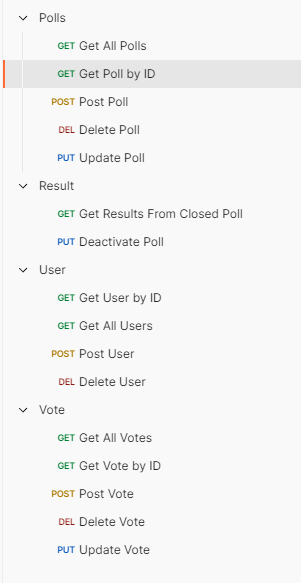
\includegraphics[width=0.3\linewidth]{figs/PostmanRequests.png}
    \caption{List of Postman requests}
    \label{fig:PostReq}
\end{figure}

Initially, our focus was to determine the range of requests that the front end of the application would execute. This investigation culminated in the identification of a series of key requests, specifically targeting Polls, Results, Users, and Votes. This comprehensive list of requests is illustrated in Figure 4, providing a clear overview of the interactions expected between the front end and the back end of our system.

\begin{figure}[!htbp]
    \centering
    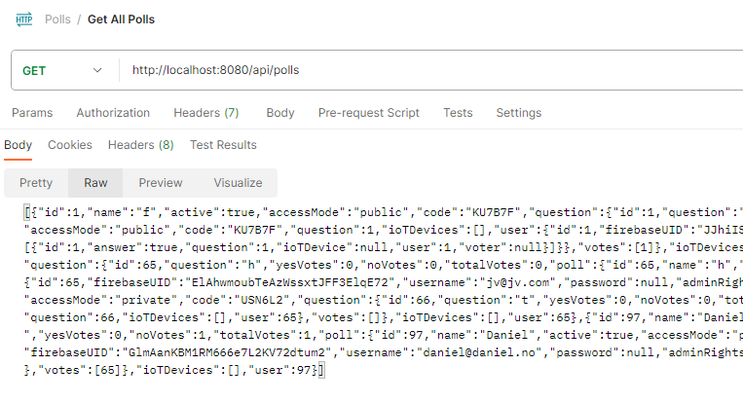
\includegraphics[width=0.5\linewidth]{figs/PostmanGetAllPolls.png}
    \caption{The request for all Polls in Postman}
    \label{fig:PostAllPolls}
\end{figure}

\begin{figure}[!htbp]
    \centering
    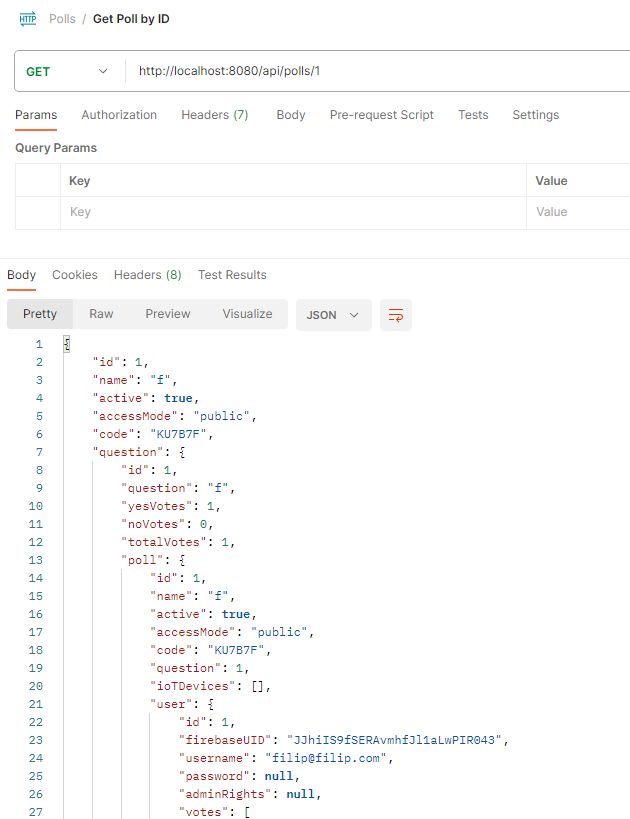
\includegraphics[width=0.5\linewidth]{figs/PostmanGetPollById.png}
    \caption{Request for a specific Poll by ID, and the resulting JSON}
    \label{fig:PostPollById}
\end{figure}

Subsequently, these identified requests were meticulously formulated and executed to monitor their respective outputs, which were primarily in JSON format. This process is exemplified in Figure 5 and Figure 6, showcasing the outcomes of different requests. The execution of these requests not only allowed for real-time observation of system responses but also led to the creation of a suite of tests. These tests could be readily deployed to evaluate the backend's functionality at any given time. This approach ensured a robustly tested and verified backend, establishing a solid foundation prior to initiating the development of the frontend.

\subsection{IDE-Based Manual Testing}

With the backend nearly complete and validated, frontend testing was conducted by running the application in the IDE. This involved using the web page to assess functionality and utilizing the IDE's debugger for in-depth testing. Regular checks and console printing were integral to this process.

\subsection{Testing Experience}

Overall, the testing experience was highly effective. Testing the backend with Postman before moving to the frontend streamlined the integration process, reducing the need for extensive backend revisions. The saved Postman requests also facilitated periodic retesting, ensuring continued backend integrity.

Frontend testing was also successful, with new features being checked alongside existing ones to maintain overall functionality. However, this manual approach to testing may become cumbersome as the application scales, indicating a potential need for automated testing in future development phases.

Regular presentations required us to thoroughly test all the old and new parts of our project, so everything ran smoothly when we showed it off. This approach really highlighted how important it is to keep testing our work carefully and consistently as we develop it.

\section{Conclusions}
\label{sec:conclusion}

Throughout the project, we embraced the challenges of learning and applying advanced technologies, each contributing uniquely to the final product.

Our adoption of React and Tailwind for the frontend infrastructure proved to be a prudent choice. React's component-based architecture greatly facilitated the creation of a dynamic and responsive user interface. The learning curve was steep but manageable, thanks in part to React's comprehensive documentation and active community support. Tailwind CSS complemented React by providing a flexible and efficient way to handle styling, which contributed to a more streamlined development process.

On the backend, Spring Boot \cite{springboot2023} stood out as a robust and scalable solution. Its maturity in the industry is evident in its comprehensive documentation and the breadth of functionalities it offers. The learning curve was somewhat challenging, particularly in mastering its extensive features and understanding the best practices for its effective use. However, the versatility and performance gains offered by Spring Boot justified the investment in learning it.

The integration of RabbitMQ \cite{rabbitmq2023} for message handling and asynchronous operations was a crucial aspect of our system's design. RabbitMQ's reliability and efficiency in handling message queues were indispensable for ensuring smooth communication and process management within our application. While its documentation was sufficient, we found that practical implementation required a deeper understanding of message queuing concepts.

Our use of Hibernate \cite{hibernate2023} and JPA for object-relational mapping and data handling significantly streamlined our interactions with the database. The ease of integration with Spring Boot and the abstraction it provided from complex database operations were particularly beneficial. Both Hibernate and JPA have mature documentation, but their learning curve can be steep for developers new to ORM concepts.

Firebase's \cite{firebase2023} integration for authentication brought a robust layer of security to our application. Its ease of use and comprehensive documentation significantly reduced the complexity typically associated with implementing authentication solutions.

In conclusion, the technology stack selected for this project not only served the immediate needs of the application but also provided a valuable learning experience. The maturity of these technologies, combined with the quality of their documentation, played a pivotal role in overcoming the initial learning curve. This project stands as a testament to the effectiveness of combining modern, robust technologies with sound design and implementation practices to create scalable, efficient, and maintainable software solutions.







\bibliographystyle{plain}
\bibliography{report.bib}{}

\end{document}
